%==================================
% SMDS TEMPLATE — Naskah Data Mining (Team LogLoss, UNITY#14)
%==================================
\documentclass[11pt,twoside]{article}

%==================================
% PACKAGES
%==================================
\usepackage{amsmath,amssymb}
\usepackage[T1]{fontenc}
\usepackage{graphicx}
\usepackage{geometry}
\geometry{margin=1in}
\usepackage[
backend=biber,
style=numeric-comp,
sorting=none,
giveninits=true,
doi=true,
url=false
]{biblatex}
\addbibresource{SMDSBib.bib}
\usepackage{fancyhdr}
\usepackage{booktabs}
\usepackage{array}
\usepackage{tikz}
\usetikzlibrary{positioning,arrows.meta,calc}
\newcommand{\shorttitle}{}
\newcommand{\shortauthor}{}
\pagestyle{fancy}
\fancyhf{}
\fancyhead[L]{\small\shorttitle}
\fancyhead[R]{\small\shortauthor}
\fancyfoot[C]{\small\thepage}

\usepackage[colorlinks=true,allcolors=blue]{hyperref}
\setlength{\emergencystretch}{2em}
\renewcommand{\abstractname}{Abstrak}
\date{19 November 2026}
\newcommand{\orcidlink}[1]{%
\href{https://orcid.org/#1}{
\includegraphics[height=1.6ex]{ORCID_iD.png}}%
}

%==================================
% SIMPLE SMDS MACROS (Compatibility Layer)
%==================================

\newcommand{\SMDStitle}[1]{\title{\bfseries #1}}
\newcommand{\SMDSshorttitle}[1]{\def\shorttitle{#1}}
\newcommand{\SMDSshortafill}[1]{\def\shortauthor{#1}}

\newcommand{\SMDSaffilone}[1]{\def\affilone{#1}}

\newcommand{\SMDSauthorone}[4]{\def\authorone{#1$^{#2}$\,\orcidlink{#3}}}
\newcommand{\SMDSauthortwo}[4]{\def\authortwo{#1$^{#2}$\,\orcidlink{#3}}}
\newcommand{\SMDSauthorthree}[4]{\def\authorthree{#1$^{#2}$\,\orcidlink{#3}}}

\newcommand{\SMDScorrespoding}[2]{%
\def\corrauthor{#1 \href{mailto:#2}{#2}}}

\newcommand{\SMDSKeywords}[1]{
\vspace{0.5em}
\noindent\textbf{Kata kunci:} #1
}

%==================================
% METADATA
%==================================

\SMDStitle{Forecasting Dampak Potensi Godzilla El Ni\~no 2026 terhadap Kekeringan Nasional Indonesia Menggunakan XGBoost dengan Rekayasa Fitur Kinematika Spatio-Temporal}

\SMDSshortafill{D. P. Akrilian dkk.}
\SMDSshorttitle{ENSO dan Kekeringan Nasional Indonesia}

\SMDSaffilone{Departemen Statistika dan Sains Data, Fakultas Matematika dan Ilmu Pengetahuan Alam, Universitas Negeri Semarang, Semarang, Indonesia}

%---------------------------------
% AUTHORS
%---------------------------------
\SMDSauthorone{Dimas Pasha Akrilian}{1}{0009-0005-6037-3591}{dimaspasha49@gmail.com}
\SMDSauthortwo{Shata Alwan Jalaluddin}{1}{0009-0007-2139-2487}{}
\SMDSauthorthree{Galih Kusuma Wijaya}{1}{0009-0002-7322-4681}{}

\SMDScorrespoding{$^*$Penulis korespondensi, email:}{dimaspasha49@gmail.com}

%==================================
% AUTHOR BLOCK
%==================================

\author{
\begin{minipage}{\textwidth}
\authorone,
\authortwo,
\authorthree
\\[1em]
$^1$ \affilone\\
\corrauthor
\end{minipage}
}

%==================================

\begin{document}

\maketitle

%==================================
\begin{abstract}
\sloppy
Sistem peringatan dini kekeringan sering mengandalkan indikator El Ni\~no--Southern Oscillation (ENSO), tetapi seberapa jauh ENSO benar-benar memprediksi kekeringan nasional Indonesia jarang diuji dengan evaluasi yang bebas kebocoran target. Kami menganalisis 312 pengamatan bulanan (2000--2025) yang menggabungkan CHIRPS, MODIS (NDVI dan LST), NOAA OISST, dan Oceanic Ni\~no Index (ONI) dengan target Standardized Drought Condition Index (SDCI). Pada rancangan awal, XGBoost dengan 72 fitur mencapai $R^2$ uji 0,80, tetapi fitur tersebut memuat NDVI, LST, dan curah hujan pada bulan yang sama, yaitu komponen penyusun SDCI. Regresi linier dari ketiganya saja menghasilkan $R^2$ uji 1,000, sehingga angka itu bukan kemampuan prediksi. Setelah komponen itu dibuang dan fitur ENSO digeser tiga bulan, XGBoost hasil optimasi Bayesian dan validasi walk-forward hanya mencapai $R^2$ uji 0,037 pada 2021--2025, sedangkan klimatologi bulanan $-0{,}051$. Korelasi silang terkuat selalu berada pada lead nol (antara $-0{,}14$ dan $-0{,}34$ menurut wilayah) dan hilang pada lead tiga bulan atau lebih; koefisien regresi ONI signifikan hanya pada lead 0 dan 1 bulan, dan uji Granger tidak signifikan pada taraf 5\%. Pengaruh bulan yang sama paling kuat di Jawa dan Nusa Tenggara. Pada skenario ONI naik linear 0,15 per bulan, SDCI nasional terendah pada September 2026 sebesar 0,529 (rentang 10--90\% 0,41--0,68), tidak lebih kering daripada rata-rata historis September. ENSO karenanya lebih berguna untuk pemantauan serempak daripada peramalan tiga bulan ke depan, dan seluruh hasil dapat direproduksi dengan seed tetap.

\end{abstract}

\SMDSKeywords{ENSO, kekeringan, SDCI, XGBoost, kebocoran target, validasi walk-forward, Godzilla El Ni\~no}

%==================================
\section{Pendahuluan}
\label{Sec:Intro}

Kekeringan akibat El Ni\~no berulang kali menekan pertanian dan memicu kebakaran lahan di Indonesia. Curah hujan Indonesia terkait kuat dengan suhu laut Pasifik tropis dan interaksi udara--laut lokal \cite{hendon2003indonesian,aldrian2003rainfall,hamada2002rainy}, dan kebakaran serta asap pada 2015 menunjukkan bahwa kekeringan yang dipicu El Ni\~no dapat berdampak nonlinear terhadap lahan gambut \cite{field2016fire}. Peristiwa 2015/2016 termasuk El Ni\~no ekstrem yang berbeda karakter dari 1997/1998 \cite{paek2017different}. Julukan ``Godzilla El Ni\~no'' dipakai untuk El Ni\~no yang sangat kuat, dan prospek kejadian serupa pada 2026 mendorong pertanyaan praktis: seberapa dini dan seberapa baik kekeringan nasional dapat diperingatkan dari indikator ENSO?

Pembelajaran mesin makin sering dipakai untuk peramalan iklim, termasuk ENSO sendiri \cite{ham2019deep}, dan model berbasis pohon seperti XGBoost \cite{chen2016xgboost} populer karena akurat pada data tabular. Namun akurasi tinggi pada data deret waktu mudah menyesatkan. Kebocoran target, yaitu fitur yang membawa informasi tentang target yang tidak tersedia saat prediksi dibuat, termasuk kesalahan yang paling sering menggelembungkan skor model \cite{kaufman2012leakage}, dan validasi silang yang mengacak urutan waktu menambah masalah yang sama \cite{bergmeir2012cv}. Pada indeks komposit seperti SDCI yang dibangun dari NDVI, suhu permukaan daratan, dan curah hujan \cite{rhee2010sdci,kogan1995vci}, memakai komponen itu sebagai prediktor sama dengan memasukkan jawaban ke dalam soal.

Penelitian ini bermula dari sistem peringatan dini berbasis XGBoost dan rekayasa fitur kinematika iklim (momentum dan akselerasi ONI) yang pada versi awalnya melaporkan $R^2$ uji 0,83. Saat mengaudit saluran fiturnya, kami menemukan bahwa angka itu berasal dari komponen penyusun SDCI. Artikel ini melaporkan temuan tersebut dan menjawab ulang pertanyaan aslinya dengan rancangan yang bebas kebocoran. Tiga kontribusi disampaikan. Pertama, kami mendemonstrasikan kebocoran target secara kuantitatif dan menunjukkan bahwa $R^2$ turun dari 0,80 ke 0,04 setelah diperbaiki. Kedua, kami mengukur struktur lead--lag antara ONI dan SDCI nasional dan regional dengan inferensi yang kokoh terhadap autokorelasi (galat Newey--West \cite{newey1987hac}) dan uji Granger \cite{granger1969causality}. Ketiga, kami membandingkan XGBoost hasil optimasi Bayesian dengan pembanding sederhana, yaitu klimatologi bulanan dan model deret waktu klasik, pada evaluasi out-of-sample, dan melaporkan secara jujur bahwa model ENSO tidak mengalahkan klimatologi pada lead tiga bulan.

Bagian~\ref{Sec:Related} meninjau penelitian terkait. Bagian~\ref{Sec:Method} menjelaskan data, rekayasa fitur, desain bebas kebocoran, dan pemodelan. Bagian~\ref{Sec:Results} melaporkan hasil, Bagian~\ref{Sec:Discussion} membahasnya beserta keterbatasannya, dan Bagian~\ref{Sec:Conclusion} menutup artikel.

%==================================
\section{Penelitian Terkait}
\label{Sec:Related}

\paragraph{ENSO dan hujan Indonesia.} Hendon \cite{hendon2003indonesian} menunjukkan bahwa ENSO memodulasi curah hujan Indonesia, dengan dampak yang menonjol pada musim kering, dan interaksi udara--laut lokal memperkuat sinyalnya. Aldrian dan Susanto \cite{aldrian2003rainfall} membagi Indonesia menjadi tiga wilayah hujan dominan dengan hubungan berbeda terhadap suhu muka laut, dan Hamada dkk.\ \cite{hamada2002rainy} mengaitkan variasi awal dan akhir musim hujan dengan ENSO. Temuan heterogenitas wilayah dalam artikel ini searah dengan gambaran tersebut, meskipun kami memakai indeks kekeringan yang dibangun dari penginderaan jauh, bukan curah hujan tunggal.

\paragraph{Indeks kekeringan berbasis satelit.} Indeks seperti Vegetation Condition Index \cite{kogan1995vci} dan indeks gabungan yang memadukan vegetasi, suhu, dan curah hujan \cite{rhee2010sdci} banyak dipakai untuk memantau kekeringan pertanian. Sifat gabungan inilah yang membuat komponen-komponennya tidak boleh dipakai sebagai prediktor indeks yang sama.

\paragraph{Pembelajaran mesin dan validasi deret waktu.} XGBoost \cite{chen2016xgboost}, LightGBM \cite{ke2017lightgbm}, dan Random Forest \cite{breiman2001rf} sering dibandingkan dengan model deret waktu klasik dan Prophet \cite{taylor2018prophet}. Untuk deret waktu, Bergmeir dan Ben\'itez \cite{bergmeir2012cv} membahas kapan validasi silang sah dipakai, sedangkan Hyndman dan Athanasopoulos \cite{hyndman2021fpp3} menekankan pembanding sederhana dan evaluasi out-of-sample. Skor keahlian terhadap klimatologi mengikuti Murphy \cite{murphy1988skill}. Penyetelan hiperparameter memakai Optuna \cite{akiba2019optuna}, dan penjelasan model memakai nilai SHAP \cite{lundberg2017shap}. Kami melengkapi literatur itu dengan studi kasus yang menunjukkan besarnya kebocoran pada indeks komposit dan dampaknya pada kesimpulan.

%==================================
\section{Metodologi}
\label{Sec:Method}

Gambar~\ref{Fig:Pipeline} meringkas alur penelitian. Analisis statistik dijalankan dalam R (korelasi silang, regresi lead, uji Granger), dan pemodelan pembelajaran mesin dalam Python (XGBoost, pembanding, dan skenario 2026). Seluruh langkah dijalankan dengan seed tetap.

\begin{figure}[ht]
\centering
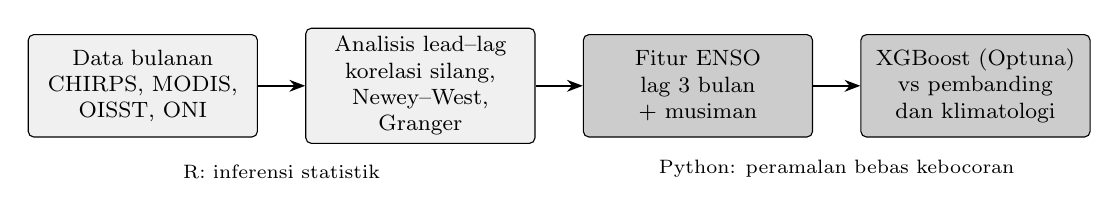
\begin{tikzpicture}[
  box/.style={draw, rounded corners=2pt, align=center, font=\footnotesize, text width=2.7cm, minimum height=13mm, inner sep=3pt},
  stat/.style={box, fill=black!6},
  ml/.style={box, fill=black!20},
  arr/.style={-{Stealth[length=2mm]}, thick},
  node distance=6mm]
\node[stat] (a) {Data bulanan\\CHIRPS, MODIS,\\OISST, ONI};
\node[stat, right=of a] (b) {Analisis lead--lag\\korelasi silang,\\Newey--West, Granger};
\node[ml, right=of b] (c) {Fitur ENSO\\lag 3 bulan\\+ musiman};
\node[ml, right=of c] (d) {XGBoost (Optuna)\\vs pembanding\\dan klimatologi};
\draw[arr] (a)--(b); \draw[arr] (b)--(c); \draw[arr] (c)--(d);
\node[font=\scriptsize] at ($(a.south)!0.5!(b.south)+(0,-4mm)$) {R: inferensi statistik};
\node[font=\scriptsize] at ($(c.south)!0.5!(d.south)+(0,-4mm)$) {Python: peramalan bebas kebocoran};
\end{tikzpicture}
\caption{Alur penelitian. Kotak terang adalah analisis statistik (R); kotak gelap adalah pemodelan pembelajaran mesin (Python).}
\label{Fig:Pipeline}
\end{figure}

\subsection{Data}
\label{SubSec:Data}

Data terdiri atas 312 pengamatan bulanan, Januari 2000 sampai Desember 2025, dengan 40 variabel numerik yang diakuisisi melalui Google Earth Engine (Tabel~\ref{Tab:Data}). Setiap variabel daratan tersedia untuk Indonesia secara nasional dan tujuh kelompok wilayah: Sumatera, Jawa, Kalimantan, Sulawesi, Nusa Tenggara, Maluku, dan Papua. Target adalah SDCI nasional (\texttt{SDCI\_Indo}), indeks gabungan dari Vegetation Condition Index (VCI), Temperature Condition Index (TCI), dan Precipitation Condition Index (PCI) yang berskala 0--1; nilai kecil menandakan kekeringan dan ambang kritis yang dipakai adalah 0,3. Sebanyak 38 sel kosong (0,3\% dari 12.480 sel) diisi dengan interpolasi berbasis waktu.

\begin{table}[ht]
\centering
\caption{Sumber data. Semua deret bulanan, 2000--2025 (312 pengamatan).}
\label{Tab:Data}
\small
\begin{tabular}{llp{6.2cm}}
\toprule
Sumber & Variabel & Keterangan \\
\midrule
CHIRPS \cite{funk2015chirps} & curah hujan & per wilayah dan nasional \\
MODIS & NDVI, LST & indeks vegetasi dan suhu permukaan daratan, per wilayah \\
NOAA OISST \cite{huang2021oisst} & SST, \textit{sst\_anomaly}, Ni\~no 1+2/3.4/4 & suhu dan anomali permukaan laut \\
NOAA & ONI \cite{trenberth1997enso} & anomali SST Ni\~no 3.4, rata-rata bergerak tiga bulan \\
Turunan & SDCI per wilayah & dari VCI, TCI, dan PCI \\
\bottomrule
\end{tabular}
\end{table}

Fase iklim ditentukan dari ONI dengan ambang $\pm 0{,}5$: 81 bulan La Ni\~na, 161 netral, dan 70 El Ni\~no. SDCI nasional berrata-rata 0,620 (simpangan baku 0,115) dan hanya lima bulan berada di bawah 0,3.

\subsection{Anomali musiman dan analisis lead--lag}
\label{SubSec:LeadLag}

SDCI sangat musiman: rata-rata bulanan menjelaskan 58,9\% variansnya, dengan nilai terendah pada Oktober (0,462) dan tertinggi pada Mei (0,744). Agar musiman tidak mengaburkan hubungan dengan ONI, kami memakai anomali $A_t = \mathrm{SDCI}_t - \overline{\mathrm{SDCI}}_{m(t)}$, yaitu selisih terhadap klimatologi bulan yang sama. Tiga analisis dilakukan pada anomali ini.

\paragraph{Korelasi silang.} Kami menghitung $\mathrm{corr}(\mathrm{ONI}_t, A_{t+h})$ untuk $h = 0,\dots,12$ bulan, per wilayah.

\paragraph{Regresi lead.} Untuk SDCI nasional, $A_{t+h} = \alpha_h + \beta_h\,\mathrm{ONI}_t + \varepsilon_{t+h}$ dengan $h = 0,\dots,9$. Galat baku memakai estimator Newey--West \cite{newey1987hac} dengan kernel Bartlett dan lag 12 tanpa prewhitening, karena galat berautokorelasi kuat pada data bulanan.

\paragraph{Uji Granger.} Kami menguji apakah ONI membantu memprediksi $A_t$ di luar riwayat $A_t$ sendiri \cite{granger1969causality} dengan orde 3, 6, dan 9. Uji ini mengukur kekuatan prediktif, bukan sebab-akibat fisis.

\subsection{Rekayasa fitur kinematika iklim}
\label{SubSec:Features}

Dari ONI dan \textit{sst\_anomaly} kami membangun 21 fitur per variabel: nilai asli, lag 1--6 dan 12 bulan, rata-rata, simpangan baku, maksimum, dan minimum bergulir (jendela 3 dan 6 bulan), rata-rata bergerak eksponensial (rentang 3 dan 6), serta fitur kinematika
\begin{equation}
v_t = x_t - x_{t-1}, \qquad v^{(3)}_t = x_t - x_{t-3}, \qquad a_t = v_t - v_{t-1},
\label{Eq:Kinematic}
\end{equation}
yang masing-masing disebut momentum (kecepatan perubahan) dan akselerasi, dengan harapan menangkap awal pemanasan Pasifik yang cepat. Dua fitur musiman, $\sin(2\pi m/12)$ dan $\cos(2\pi m/12)$, ditambahkan. Hasilnya 44 fitur.

\subsection{Rancangan bebas kebocoran}
\label{SubSec:Leakfree}

Versi awal studi memakai 72 fitur: fitur ENSO di atas ditambah semua variabel daratan (NDVI, LST, curah hujan, \textit{Suhu\_Permukaan\_C}, \textit{Curah\_Hujan\_mm}) pada bulan yang sama dengan target. Karena SDCI dibangun dari NDVI, LST, dan curah hujan, rancangan itu membocorkan target. Rancangan bebas kebocoran memakai tiga aturan.
\begin{enumerate}
\item Variabel penyusun SDCI pada bulan target tidak dipakai. Prediktor hanya turunan ONI dan \textit{sst\_anomaly} yang digeser $H = 3$ bulan, yaitu fitur sampai bulan $t - 3$ memprediksi SDCI bulan $t$, ditambah dua fitur musiman yang diketahui untuk bulan target.
\item Pembagian data kronologis 80/20: 237 bulan latih (April 2001--Desember 2020) dan 60 bulan uji (Januari 2021--Desember 2025). Data uji tidak disentuh saat penyetelan maupun saat berhenti dini (\textit{early stopping}), yang memakai 15\% ekor data latih sebagai validasi.
\item Semua model dibandingkan pada fitur dan pembagian yang sama, dan klimatologi bulanan (rata-rata SDCI per bulan dari data latih) dilaporkan sebagai pembanding utama.
\end{enumerate}

\subsection{Pemodelan}
\label{SubSec:Models}

XGBoost \cite{chen2016xgboost} dengan objektif kuadrat terkecil disetel oleh optimasi Bayesian Optuna \cite{akiba2019optuna}: 50 percobaan, sampler TPE dengan seed 42, dan MedianPruner. Fungsi objektifnya adalah rata-rata RMSE pada validasi walk-forward lima lipatan (\texttt{TimeSeriesSplit}) di dalam data latih. Ruang pencarian memuat jumlah pohon (100--500), kedalaman (3--9), laju belajar ($0{,}005$--$0{,}1$, skala log), \textit{subsample} dan \textit{colsample} (0,5--0,9), bobot anak minimum (1--10), regularisasi L1 dan L2 ($10^{-3}$--10), dan $\gamma$ ($10^{-3}$--1). Pembanding adalah ARIMA(1,1,1), Prophet \cite{taylor2018prophet}, Random Forest \cite{breiman2001rf}, LightGBM \cite{ke2017lightgbm}, XGBoost dengan parameter bawaan, dan klimatologi bulanan.

Untuk skenario 2026, tiga model XGBoost kuantil (objektif \textit{pinball loss} \cite{koenker1978quantile} pada kuantil 0,1; 0,5; dan 0,9) dilatih pada fitur turunan ONI dan musiman. Skenario mengasumsikan ONI naik linear 0,15 per bulan selama dua belas bulan dari nilai terakhir (Desember 2025: $-0{,}60$). Jalur ini asumsi, bukan prakiraan ONI.

\subsection{Metrik dan reprodusibilitas}
\label{SubSec:Metrics}

Kami melaporkan RMSE, MAE, dan koefisien determinasi uji $R^2 = 1 - \sum (y_t - \hat y_t)^2 / \sum (y_t - \bar y)^2$. Untuk evaluasi out-of-sample dengan jendela meluas, kami memakai skor keahlian $1 - \mathrm{MSE}_{\mathrm{ONI}} / \mathrm{MSE}_{\mathrm{klim}}$ terhadap klimatologi \cite{murphy1988skill}, yang bernilai positif bila model ENSO lebih baik daripada klimatologi. Seluruh kode dijalankan dengan seed 42 (sampler Optuna, \texttt{numpy}, dan \texttt{random}); dua run berurutan pada platform Kaggle menghasilkan berkas hasil yang identik.

%==================================
\section{Hasil Empiris}
\label{Sec:Results}

\subsection{Pola umum SDCI dan ONI}
\label{SubSec:Overview}

Gambar~\ref{Fig:TS} memperlihatkan anomali SDCI nasional dan ONI. SDCI terendah sepanjang periode terjadi pada Oktober 2015 (0,013), menjelang ONI mencapai puncaknya pada Desember 2015 (2,62), saat El Ni\~no 2015/2016 berkembang. Korelasi mentah antara ONI dan SDCI hanya $-0{,}19$. Rata-rata SDCI pada fase El Ni\~no (0,568) lebih rendah daripada fase netral (0,646) dan La Ni\~na (0,614), tetapi simpangan bakunya paling besar (0,142), sehingga distribusinya lebar dan tumpang tindih.

\begin{figure}[ht]
\centering
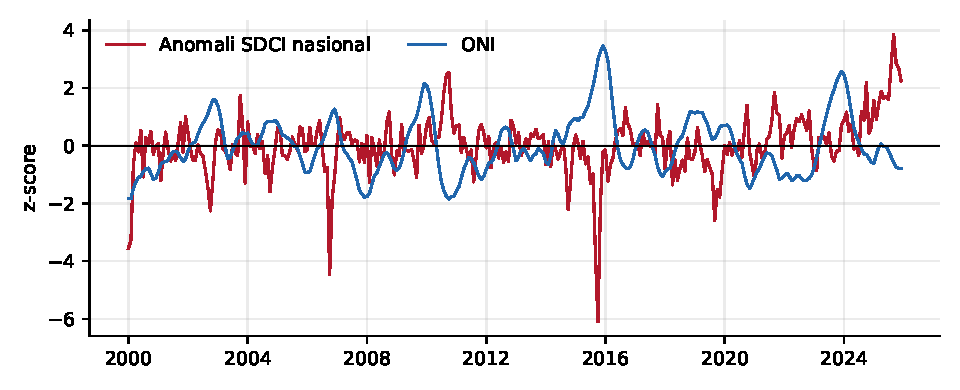
\includegraphics[width=0.85\textwidth]{figs/fig_ts.pdf}
\caption{Anomali SDCI nasional dan ONI (keduanya distandardisasi). Penurunan SDCI terjadi bersamaan dengan El Ni\~no kuat, tetapi puncak ONI tidak selalu diikuti penurunan SDCI yang sebanding.}
\label{Fig:TS}
\end{figure}

\subsection{Struktur lead--lag}
\label{SubSec:Lag}

Gambar~\ref{Fig:CC} menyajikan korelasi silang per wilayah. Di setiap wilayah, korelasi negatif terkuat berada pada lead nol dan melemah dengan cepat sejalan bertambahnya lead; tidak ada bukti dampak tertunda beberapa bulan. Nilainya berkisar dari $-0{,}14$ (Papua) sampai $-0{,}34$ (Nusa Tenggara); nasional $-0{,}29$.

\begin{figure}[ht]
\centering
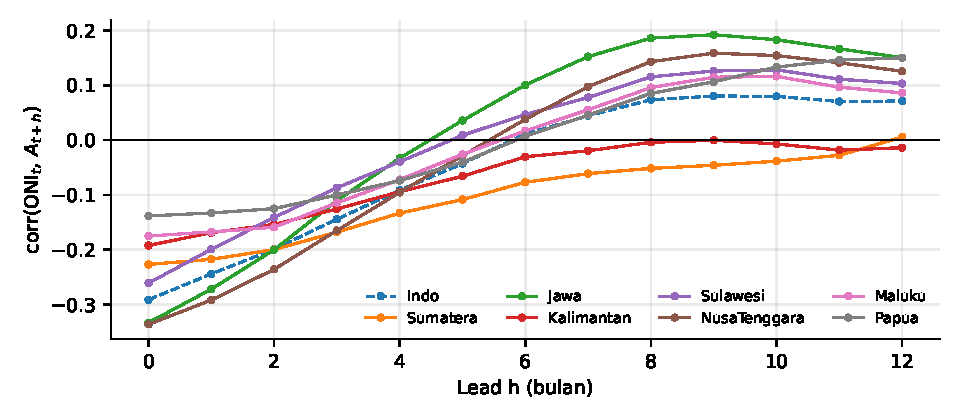
\includegraphics[width=0.85\textwidth]{figs/fig_cc.pdf}
\caption{Korelasi silang antara ONI pada bulan $t$ dan anomali SDCI pada bulan $t+h$. Garis putus-putus adalah SDCI nasional.}
\label{Fig:CC}
\end{figure}

Tabel~\ref{Tab:Lead} dan Gambar~\ref{Fig:Beta} melaporkan regresi lead nasional. Koefisien ONI signifikan pada lead 0 ($\hat\beta = -0{,}028$, $p = 0{,}021$) dan lead 1 ($-0{,}023$, $p = 0{,}032$), batas pada lead 2 ($p = 0{,}053$), dan tidak signifikan dari lead 3 ke atas. Koefisien berbalik tanda pada lead 6 ke atas, tetapi dengan galat baku yang lebih besar daripada nilainya. $R^2$ tertinggi hanya 0,085, yaitu ONI menjelaskan kurang dari sepersepuluh variasi anomali SDCI bulan yang sama. Uji Granger tidak signifikan pada taraf 5\%: $p = 0{,}091$ (orde 3), 0,154 (orde 6), dan 0,051 (orde 9).

\begin{table}[ht]
\centering
\caption{Regresi lead anomali SDCI nasional pada ONI: $A_{t+h} = \alpha_h + \beta_h\,\mathrm{ONI}_t$. Galat baku Newey--West (lag 12); $n = 312 - h$.}
\label{Tab:Lead}
\small
\begin{tabular}{rrrrr}
\toprule
$h$ (bulan) & $\hat\beta_h$ & Galat baku & Nilai $p$ & $R^2$ \\
\midrule
0 & $-0{,}0282$ & 0,0122 & 0,021 & 0,085 \\
1 & $-0{,}0232$ & 0,0108 & 0,032 & 0,060 \\
2 & $-0{,}0186$ & 0,0096 & 0,053 & 0,040 \\
3 & $-0{,}0135$ & 0,0087 & 0,121 & 0,021 \\
4 & $-0{,}0086$ & 0,0082 & 0,298 & 0,008 \\
5 & $-0{,}0040$ & 0,0082 & 0,623 & 0,002 \\
6 & $0{,}0010$ & 0,0084 & 0,902 & 0,000 \\
7 & $0{,}0041$ & 0,0088 & 0,640 & 0,002 \\
8 & $0{,}0069$ & 0,0092 & 0,457 & 0,005 \\
9 & $0{,}0075$ & 0,0094 & 0,425 & 0,007 \\
\bottomrule
\end{tabular}
\end{table}

\begin{figure}[ht]
\centering
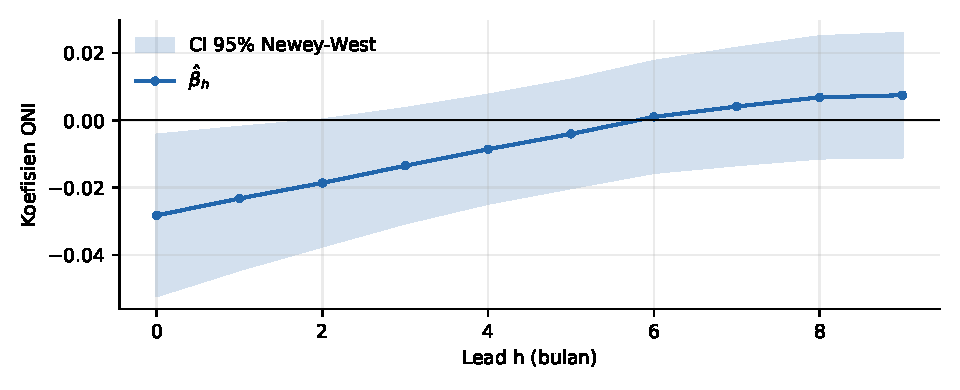
\includegraphics[width=0.85\textwidth]{figs/fig_beta.pdf}
\caption{Koefisien ONI pada anomali SDCI nasional menurut lead, dengan pita kepercayaan 95\% Newey--West. Pita memuat nol dari lead 2.}
\label{Fig:Beta}
\end{figure}

\subsection{Heterogenitas wilayah}
\label{SubSec:Regions}

Tabel~\ref{Tab:Regions} menunjukkan bahwa koefisien ONI pada lead nol bernilai negatif di semua wilayah, tetapi kekuatannya berbeda. Nusa Tenggara ($-0{,}038$, $p = 0{,}001$) dan Jawa ($-0{,}035$, $p = 0{,}0005$) paling sensitif, dengan $R^2$ sekitar 0,11. Sulawesi dan Sumatera signifikan pada taraf 5\% tetapi tidak setelah koreksi Bonferroni untuk delapan wilayah ($\alpha = 0{,}00625$), sedangkan Kalimantan, Maluku, dan Papua tidak signifikan. Hanya Jawa dan Nusa Tenggara yang tetap signifikan setelah koreksi.

\begin{table}[ht]
\centering
\caption{Regresi lead 0 anomali SDCI per wilayah pada ONI (galat baku Newey--West). Koreksi Bonferroni untuk delapan wilayah: $\alpha = 0{,}00625$.}
\label{Tab:Regions}
\small
\begin{tabular}{lrrr}
\toprule
Wilayah & $\hat\beta_0$ & Nilai $p$ & $R^2$ \\
\midrule
Nusa Tenggara & $-0{,}0383$ & 0,0010 & 0,113 \\
Jawa          & $-0{,}0354$ & 0,0005 & 0,111 \\
Indonesia     & $-0{,}0282$ & 0,0212 & 0,085 \\
Sulawesi      & $-0{,}0240$ & 0,0095 & 0,068 \\
Sumatera      & $-0{,}0207$ & 0,0496 & 0,052 \\
Kalimantan    & $-0{,}0191$ & 0,1537 & 0,037 \\
Maluku        & $-0{,}0171$ & 0,1379 & 0,031 \\
Papua         & $-0{,}0111$ & 0,2058 & 0,019 \\
\bottomrule
\end{tabular}
\end{table}

\subsection{Demonstrasi kebocoran target}
\label{SubSec:Leak}

Gambar~\ref{Fig:Leak} dan Tabel~\ref{Tab:Leak} merangkum eksperimen inti. Regresi linier SDCI nasional pada NDVI, LST, dan curah hujan nasional bulan yang sama menghasilkan $R^2$ uji sebesar 1,000 (pembagian kronologis 80/20 pada 312 bulan), yang berarti SDCI adalah fungsi hampir deterministik dari ketiganya. Bila ONI dan \textit{sst\_anomaly} bulan yang sama dipakai tanpa komponen itu, $R^2$ uji adalah $-0{,}373$. Rancangan awal dengan 72 fitur memperoleh $R^2$ uji 0,80 pada XGBoost hasil penyetelan, dan laporan versi awal bahkan mencatat 0,83; kedua angka itu semata-mata mencerminkan fitur penyusun SDCI.

\begin{figure}[ht]
\centering
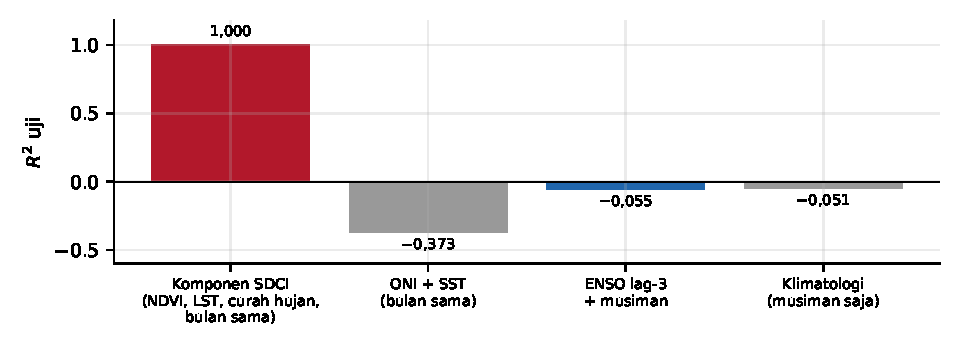
\includegraphics[width=0.85\textwidth]{figs/fig_leak.pdf}
\caption{$R^2$ uji model linier untuk SDCI nasional menurut himpunan prediktor. Komponen penyusun SDCI pada bulan yang sama merekonstruksi target hampir sempurna, sedangkan prediktor ENSO yang sah tidak mengalahkan klimatologi.}
\label{Fig:Leak}
\end{figure}

\begin{table}[ht]
\centering
\caption{$R^2$ uji model linier SDCI nasional. Baris 1--2: pembagian 80/20 pada 312 bulan (uji 63 bulan). Baris 3--4: sampel bebas kebocoran dengan lead 3 bulan, 297 bulan (uji 60 bulan, 2021--2025).}
\label{Tab:Leak}
\small
\begin{tabular}{lr}
\toprule
Prediktor & $R^2$ uji \\
\midrule
NDVI, LST, curah hujan nasional (bulan yang sama) & 1,000 \\
ONI + \textit{sst\_anomaly} (bulan yang sama) & $-0{,}373$ \\
ENSO lag 3 bulan + musiman (OLS) & $-0{,}055$ \\
Klimatologi bulanan & $-0{,}051$ \\
\bottomrule
\end{tabular}
\end{table}

\subsection{Evaluasi out-of-sample dengan jendela meluas}
\label{SubSec:OOS}

Untuk menghindari ketergantungan pada satu pembagian, kami mengevaluasi model $y_t = \alpha + \beta\,\mathrm{ONI}_{t-h} + \gamma_{m(t)}$ secara rekursif: setiap bulan uji (2021 sampai 2025) diprediksi hanya dengan pasangan data yang sudah tersedia saat itu, lalu dibandingkan dengan klimatologi. Tabel~\ref{Tab:OOS} menunjukkan skor keahlian negatif pada semua lead yang diuji (1, 3, 6, dan 9 bulan): menambahkan ONI justru sedikit memperbesar galat dibanding klimatologi, dengan selisih RMSE sangat kecil (kurang dari 0,001 pada lead 3).

\begin{table}[ht]
\centering
\caption{Evaluasi out-of-sample jendela meluas (bulan uji 2021--2025). Skor keahlian $1 - \mathrm{MSE}_{\mathrm{ONI}}/\mathrm{MSE}_{\mathrm{klim}}$; nilai negatif berarti model ONI lebih buruk daripada klimatologi.}
\label{Tab:OOS}
\small
\begin{tabular}{rrrrr}
\toprule
Lead (bulan) & $n$ uji & RMSE ONI+musiman & RMSE klimatologi & Skor keahlian \\
\midrule
1 & 62 & 0,0933 & 0,0933 & $-0{,}0017$ \\
3 & 60 & 0,0869 & 0,0862 & $-0{,}0173$ \\
6 & 57 & 0,0726 & 0,0724 & $-0{,}0038$ \\
9 & 54 & 0,0675 & 0,0674 & $-0{,}0015$ \\
\bottomrule
\end{tabular}
\end{table}

\subsection{XGBoost dan pembanding pada fitur bebas kebocoran}
\label{SubSec:ML}

Tabel~\ref{Tab:Bench} dan Gambar~\ref{Fig:Bench} membandingkan semua model pada 44 fitur bebas kebocoran dan lead tiga bulan (uji 60 bulan). XGBoost hasil optimasi Bayesian mencapai RMSE terbaik (0,0951) dan $R^2$ uji 0,037, satu-satunya yang positif. Itu jauh dari 0,80 pada rancangan awal. LightGBM ($-0{,}004$), Random Forest ($-0{,}023$), dan klimatologi ($-0{,}051$) berada di sekitar nol, XGBoost bawaan $-0{,}170$, Prophet $-0{,}430$, dan ARIMA $-1{,}099$. Selisih XGBoost hasil penyetelan terhadap klimatologi (RMSE 0,0951 dibanding 0,0993) kecil dan kami tidak menguji signifikansinya; dengan 60 bulan uji yang berautokorelasi, selisih ini belum cukup untuk menyimpulkan keunggulan. RMSE validasi walk-forward terbaik adalah 0,0686 (percobaan ke-47, 209 iterasi), dibanding 0,0701 untuk klimatologi pada lipatan yang sama; XGBoost lebih baik pada tiga dari lima lipatan dan lebih buruk pada dua. $R^2$ per lipatan XGBoost berkisar 0,43--0,81 tetapi sebagian besar mencerminkan musiman, karena klimatologi saja mencapai 0,12--0,81 pada lipatan yang sama. Nilai $R^2$ negatif sebagian dipicu pergeseran level: rata-rata SDCI pada periode uji 0,673 lebih tinggi daripada data latih (0,610), dan periode uji memuat El Ni\~no 2023 (ONI puncak 1,95) dengan SDCI terendah 0,447.

\begin{table}[ht]
\centering
\caption{Kinerja uji (2021--2025, 60 bulan) pada fitur ENSO lag 3 bulan + musiman. XGBoost (Optuna) dan pembanding memakai pembagian dan fitur yang sama. MAE XGBoost hasil penyetelan tidak direkam.}
\label{Tab:Bench}
\small
\begin{tabular}{lrrr}
\toprule
Model & RMSE & MAE & $R^2$ \\
\midrule
XGBoost (Optuna)    & \textbf{0,0951} & --     & \textbf{0,0374} \\
LightGBM            & 0,0971 & 0,0716 & $-0{,}0036$ \\
Random Forest       & 0,0980 & 0,0764 & $-0{,}0228$ \\
Klimatologi bulanan & 0,0993 & 0,0746 & $-0{,}0505$ \\
XGBoost (bawaan)    & 0,1048 & 0,0783 & $-0{,}1697$ \\
Prophet             & 0,1159 & 0,0914 & $-0{,}4297$ \\
ARIMA(1,1,1)        & 0,1404 & 0,1189 & $-1{,}0989$ \\
\bottomrule
\end{tabular}
\end{table}

\begin{figure}[ht]
\centering
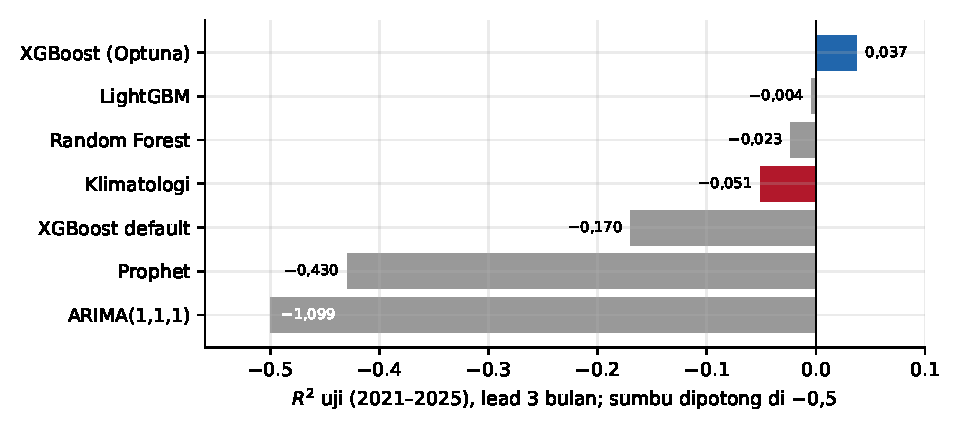
\includegraphics[width=0.85\textwidth]{figs/fig_bench.pdf}
\caption{$R^2$ uji menurut model pada rancangan bebas kebocoran. Hanya XGBoost hasil penyetelan yang positif, dan nilainya hampir nol.}
\label{Fig:Bench}
\end{figure}

\subsection{Reprodusibilitas}
\label{SubSec:Repro}

Pada rancangan awal tanpa seed, lima run berurutan menghasilkan percobaan terbaik yang berbeda (nomor 31 sampai 49) dan $R^2$ uji antara 0,776 dan 0,821, karena sampler Optuna bersifat acak; lima run dengan seed 42 identik seluruhnya. Pada rancangan bebas kebocoran, dua run dengan seed 42 menghasilkan berkas hasil yang identik byte demi byte. Angka yang dilaporkan di sini karenanya dapat direproduksi, tetapi angka versi awal (0,8044 pada keluaran notebook dan 0,8257 pada laporan) tidak, karena berasal dari run tanpa seed.

\subsection{Skenario Godzilla El Ni\~no 2026}
\label{SubSec:Scenario}

Dengan jalur ONI yang diasumsikan naik 0,15 per bulan, ONI mencapai sekitar $+1{,}2$ pada Desember 2026, yaitu El Ni\~no sedang, belum sekuat 2015. Model kuantil memproyeksikan SDCI nasional terendah pada September 2026 sebesar 0,529 dengan rentang 10--90\% sebesar 0,410--0,676. Nilai ini masih di dalam rentang historis normal, jauh di atas ambang kritis 0,3, dan sedikit di atas rata-rata historis September (0,493). Hasil ini konsisten dengan temuan Bagian~\ref{SubSec:ML}: model berbasis ONI lag tiga bulan hampir tidak bergeser dari pola musiman, sehingga proyeksi itu tidak dapat dibaca sebagai sinyal kekeringan ekstrem.

%==================================
\section{Diskusi}
\label{Sec:Discussion}

\paragraph{Kebocoran target adalah temuan utama.} Perbedaan antara $R^2$ 0,80 dan 0,04 sepenuhnya berasal dari satu keputusan desain: menyertakan variabel yang membentuk target. Ini sejalan dengan peringatan Kaufman dkk.\ \cite{kaufman2012leakage} bahwa kebocoran sulit dikenali justru karena skor modelnya tampak bagus. Pemeriksaan yang cukup murah adalah meregresikan target pada kandidat prediktor secara linier: $R^2$ mendekati 1 sudah menjadi tanda bahaya. Pada indeks komposit, aturan praktisnya adalah memperlakukan komponen indeks sebagai bagian dari target.

\paragraph{ENSO memberi sinyal serempak, bukan peringatan dini tiga bulan.} Korelasi dan koefisien ONI terkuat pada lead nol dan menghilang pada lead tiga bulan atau lebih. Ini searah dengan gambaran bahwa ENSO memodulasi curah hujan Indonesia secara cepat melalui sirkulasi atmosfer dan interaksi udara--laut lokal \cite{hendon2003indonesian,aldrian2003rainfall}, bukan melalui penundaan beberapa bulan. Namun besar efeknya kecil terhadap variasi anomali SDCI (maksimum $R^2$ 0,085), karena sebagian besar variasi SDCI berasal dari musiman (58,9\%) dan faktor lain yang tidak dimodelkan. Akibatnya, sistem peringatan dini yang hanya mengandalkan ONI tiga bulan sebelumnya tidak memberi keunggulan atas klimatologi.

\paragraph{Heterogenitas wilayah.} Jawa dan Nusa Tenggara paling sensitif dan tetap signifikan setelah koreksi pengujian berganda, sedangkan Papua, Maluku, dan Kalimantan lemah. Pola ini searah dengan perbedaan wilayah hujan yang dilaporkan sebelumnya \cite{aldrian2003rainfall,hamada2002rainy}, tetapi kami tidak menguji penyebabnya. Indeks nasional merata-ratakan delapan wilayah dengan sensitivitas berbeda, sehingga sinyal nasional lebih lemah daripada sinyal wilayah paling responsif. Peringatan dini yang fokus pada Jawa dan Nusa Tenggara kemungkinan lebih bermakna.

\paragraph{Kegunaan fitur kinematika.} Momentum dan akselerasi ONI dirancang untuk mendeteksi pemanasan cepat sebelum El Ni\~no matang. Pada data ini, fitur itu tidak menghasilkan keunggulan terukur atas klimatologi pada lead tiga bulan. Kami tidak menguji apakah fitur kinematika berguna untuk meramalkan ONI itu sendiri, yang merupakan tujuan lain.

\paragraph{Implikasi untuk peringatan dini.} Hasil ini mendukung penggunaan ENSO sebagai pemantau serempak dan konteks, dan tidak mendukung klaim bahwa model yang dilatih pada ONI lag tiga bulan dapat memperingatkan kekeringan nasional. Peningkatan kemungkinan datang dari prediktor tambahan (misalnya Indian Ocean Dipole, kelembapan tanah, dan persistensi SDCI sendiri) dan dari target regional.

\paragraph{Keterbatasan.} (1) Target adalah satu indeks nasional yang dirata-ratakan dari delapan wilayah. (2) Data hanya 312 bulan dan uji hanya 60 bulan, sehingga selisih kecil antarmodel tidak dapat dibedakan dari derau, dan nilai $p$ Newey--West bersifat asimtotik. (3) Persistensi SDCI (SDCI yang di-lag) tidak diuji sebagai prediktor, padahal pembanding ini kemungkinan kuat. (4) Pembanding ARIMA dan Prophet tidak disetel. (5) Rata-rata SDCI pada periode uji bergeser dari data latih (0,673 dibanding 0,610), yang menekan $R^2$ semua model. (6) Skenario 2026 bergantung pada jalur ONI asumsi yang hanya mencapai $+1{,}2$, jadi bukan simulasi El Ni\~no ekstrem. (7) Rumusan SDCI mengikuti definisi proyek; kami tidak membandingkannya dengan pembobotan lain. (8) MAE XGBoost hasil penyetelan tidak tercatat.

%==================================
\section{Kesimpulan}
\label{Sec:Conclusion}

Kami menguji seberapa jauh ENSO memprediksi kekeringan nasional Indonesia dengan data bulanan 2000--2025. Rancangan awal yang melaporkan $R^2$ uji sekitar 0,80 ternyata bocor: NDVI, LST, dan curah hujan bulan yang sama merekonstruksi SDCI dengan $R^2$ uji 1,000. Setelah komponen itu dibuang dan fitur ENSO digeser tiga bulan, XGBoost hasil penyetelan hanya mencapai $R^2$ uji 0,037 (RMSE 0,0951), dan klimatologi bulanan $-0{,}051$ (RMSE 0,0993). Skor keahlian ONI terhadap klimatologi negatif pada lead 1, 3, 6, dan 9 bulan. ONI berkorelasi negatif dengan SDCI pada bulan yang sama dan satu bulan sesudahnya, paling kuat di Jawa dan Nusa Tenggara, tetapi hubungan itu hilang pada lead tiga bulan atau lebih dan hanya menjelaskan kurang dari sepersepuluh variasi anomali. Pada skenario ONI naik linear, SDCI nasional September 2026 diproyeksikan 0,529 (rentang 10--90\% 0,41--0,68), tidak lebih kering daripada rata-rata historis. Dalam praktik, ENSO layak dipakai sebagai pemantau serempak kekeringan di Jawa dan Nusa Tenggara, tetapi bukan sebagai prediktor tunggal tiga bulan ke depan. Pemeriksaan kebocoran target, pembanding klimatologi, dan seed tetap sebaiknya menjadi praktik baku dalam studi peringatan dini serupa.

%==================================

\printbibliography[title={Daftar Pustaka}]

%==================================
\appendix

\section{Ketersediaan Data dan Kode}
\label{Sec:SuppA}

\sloppy
Data bulanan (312 baris) berada di \texttt{data/master\_dataset\_godzilla\_elnino\_2000\_2025.csv}. Notebook \texttt{notebooks/godzila-el-nino.ipynb} memuat seluruh pemodelan Python dan, pada sel terakhirnya, analisis R. Analisis R yang sama tersedia sebagai dokumen R Markdown \texttt{R/analisis\_R.Rmd} (hasil render \texttt{docs/analisis\_R.html}). Skrip \texttt{artikel\_smds/buat\_figur.py} membuat ulang semua gambar dan menghitung ulang tabel lead--lag dengan implementasi Newey--West sendiri; hasilnya cocok dengan R untuk semua lead. Angka XGBoost dan pembanding (Tabel~\ref{Tab:Bench}) disalin dari keluaran kernel Kaggle ber-seed dan disimpan di \texttt{artikel\_smds/hasil\_kaggle\_seeded.json}. Seed yang dipakai adalah 42.

\end{document}
